\chapter{Metodología}
\label{chap:meth}

La presente investigación sigue un enfoque experimental y cuantitativo, estructurado en seis fases: (i) construcción del pipeline de datos, (ii) entrenamiento y comparación offline de modelos livianos, (iii) implementación de la arquitectura jerárquica de aprendizaje federado, (iv) integración de cifrado ligero ASCON-128, (v) construcción de una línea base sin cifrado y (vi) evaluación de variantes con MLP/RN, CNN-1D y estrategia FOG sobre hardware real.

% ====================================================================
\section{Modelo de Amenazas y Suposiciones}
\label{sec:threat_model}

Antes de detallar la arquitectura, se hace explícito el modelo de amenazas que motiva las decisiones de diseño. Se asume un atacante de red pasivo o activo capaz de observar y modificar el tráfico inalámbrico entre nodos ESP32, gateways Raspberry Pi y el PC coordinador, pero \emph{externo} al sistema. Las amenazas que el sistema busca mitigar son:

\begin{itemize}
    \item \textbf{Confidencialidad de pesos y features:} Un atacante que capture los mensajes MQTT/HTTP no debe poder leer el contenido (pesos federados, métricas locales, vectores de features). Esto se garantiza con ASCON-128 sobre todos los canales \cite{NISTSP8002322025, Kaur2025_ASCON_Survey}.
    \item \textbf{Integridad y autenticidad:} Mensajes alterados o inyectados deben ser detectados y descartados. Se usa el tag de autenticación de 128 bits que ASCON-128 produce de forma nativa, evitando el patrón frecuente de combinar cifrado simétrico con HMAC externo \cite{NISTIR8454_2023}.
    \item \textbf{Reuso de mensajes (replay):} Cada nonce se construye a partir de un timestamp truncado a 32 bits y un contador monótono local; combinado con el tag autenticado, esto detecta reutilizaciones aunque un atacante reenvíe un mensaje válido.
    \item \textbf{Diseños criptográficos no estandarizados:} Se descarta el uso de permutaciones ultra-ligeras \emph{ad-hoc} para autenticación, dado que análisis recientes han demostrado vulnerabilidades estructurales explotables sobre Raspberry Pi en condiciones realistas \cite{Mirzaali2025_LWC_Permutations}.
\end{itemize}

\noindent\textbf{Amenazas fuera del alcance.} Se delimitan explícitamente las siguientes amenazas que \emph{no} se mitigan en esta versión del sistema:

\begin{itemize}
    \item \textbf{Clientes bizantinos / data poisoning:} Un gateway o nodo edge comprometido podría enviar pesos manipulados que sesguen el modelo global. La literatura reporta que un 10\% de participantes maliciosos puede degradar la accuracy global de 96\% a 23\% \cite{Tran2026_EdgeTrustShard}. Mitigaciones (Krum, FLTrust, Fed-NGA, MF-PoP) requieren capacidades de cómputo y memoria que exceden las de un MCU sin descomposición arquitectónica adicional. Esta línea queda como trabajo futuro.
    \item \textbf{Ataques de canal lateral sobre ASCON:} Análisis de potencia, EM o fault injection contra la implementación ASCON pueden recuperar la clave si el atacante tiene acceso físico al MCU \cite{Kaur2025_ASCON_Survey}. El sistema asume despliegue en un entorno físico controlado.
    \item \textbf{Inferencia de membresía:} Aunque FL no comparte datos crudos, los pesos pueden filtrar información sobre los datos locales. Defensas como differential privacy (DP-SGD) no se aplican en esta versión.
    \item \textbf{Compromiso del PC coordinador:} El PC se asume confiable (TCB). Trabajos basados en blockchain o multi-coordinador podrían eliminar este supuesto \cite{Tran2026_EdgeTrustShard}.
\end{itemize}


% ====================================================================
\section{Arquitectura del Sistema}
\label{sec:arquitectura}

El sistema propuesto se organiza en tres capas jerárquicas que reflejan la topología Edge--Fog--Cloud, cada una con roles diferenciados de procesamiento, entrenamiento y coordinación.

\subsection{Capa Edge: Nodos ESP32-S3}

Los nodos de borde se implementan sobre microcontroladores \textbf{ESP32-S3} con conectividad Wi-Fi nativa. Cada nodo cumple tres funciones:
\begin{enumerate}
    \item \textbf{Generación y captura de tráfico:} simula flujos de red MQTT con patrones estadísticos calibrados a partir de los datasets reales (Sección~\ref{sec:dataset}).
    \item \textbf{Extracción de características:} computa en tiempo real un vector de 13 features por flujo (Tabla~\ref{tab:features}).
    \item \textbf{Inferencia local (TinyML):} ejecuta un modelo compacto directamente en el microcontrolador, clasificando cada flujo en tres categorías: \texttt{normal}, \texttt{mqtt\_bruteforce} y \texttt{scan\_A}.
\end{enumerate}

Se despliegan dos nodos diferenciados: un nodo \emph{normal} que genera exclusivamente tráfico benigno, y un nodo \emph{simulado} que genera una mezcla de 40\% normal, 30\% bruteforce y 30\% scan\_A, reproduciendo las distribuciones estadísticas reales de los datasets. En la rama RN se usa un MLP; en la rama CNN se usa una CNN-1D con capas convolucionales fijas y capas densas federadas.

\subsection{Capa Fog: Gateway Raspberry Pi 4}

La Raspberry Pi 4 actúa como \emph{gateway} Fog y ejecuta \texttt{gateway\_hfl.py} o \texttt{gateway\_hfl\_fog.py}, según el escenario experimental. Sus responsabilidades incluyen:
\begin{itemize}
    \item Actuar como \textbf{broker MQTT} (Mosquitto) para recibir las features de los ESP32.
    \item Mantener un \textbf{buffer de entrenamiento} de $N_s = 40$ muestras etiquetadas mediante una función heurística basada en las distribuciones reales del dataset.
    \item \textbf{Entrenar localmente} un modelo Keras/TensorFlow idéntico al del ESP32 (5 épocas, Adam con $\eta=0.005$, batch=8).
    \item \textbf{Transmitir los pesos} de las capas federadas al servidor central vía HTTP.
    \item \textbf{Distribuir el modelo global} recibido del servidor a los ESP32 vía MQTT.
    \item En modo FOG, \textbf{agregar pesos entre gateways Raspberry Pi} antes de enviar una actualización preagregada al PC.
\end{itemize}

\subsection{Capa Cloud: Servidor PC}

Un PC convencional ejecuta \texttt{server\_hfl.py} o \texttt{server\_hfl\_fog.py} (FastAPI + Uvicorn) y coordina el aprendizaje federado global:
\begin{itemize}
    \item Recibe los pesos locales de $K$ gateways (en esta implementación, $K=2$).
    \item Aplica el algoritmo \textbf{FedAvg} (Sección~\ref{sec:fedavg}) ponderado por número de muestras.
    \item Distribuye el modelo global actualizado a todos los gateways.
    \item Proporciona un \textbf{dashboard analítico} en tiempo real con gráficas de accuracy y loss por ronda.
\end{itemize}

\subsection{Modos de operación}

La versión \texttt{hfl\_v7} fue implementada en dos modos:
\begin{itemize}
    \item \textbf{Modo estándar:} cada Raspberry Pi actúa como gateway independiente. El servidor PC espera actualizaciones de $K=2$ gateways y aplica FedAvg global.
    \item \textbf{Modo FOG:} una Raspberry Pi líder recibe pesos de una Raspberry Pi par mediante MQTT, calcula FedAvg local de la capa fog y envía al PC una actualización preagregada. El modelo global retorna al líder y se redistribuye a los peers y a los ESP32.
\end{itemize}

% ====================================================================
\section{Conjunto de Datos}
\label{sec:dataset}

Se utilizan tres datasets públicos de flujos de red IoT, cada uno representando una clase de tráfico. Estos provienen de capturas PCAP procesadas y convertidas a representaciones de flujo unidireccional (\emph{uniflow}):

\begin{table}[H]
\centering
\caption{Composición del dataset de flujos de red.}
\label{tab:dataset_comp}
\begin{tabular}{l r r l}
\toprule
\textbf{Dataset} & \textbf{Flujos} & \textbf{Etiqueta} & \textbf{Protocolo principal} \\
\midrule
\texttt{uniflow\_normal.csv}           & 171\,837 & 0 (\texttt{normal})           & MQTT, TCP \\
\texttt{uniflow\_mqtt\_bruteforce.csv} &  33\,080 & 1 (\texttt{mqtt\_bruteforce}) & MQTT (login) \\
\texttt{uniflow\_scan\_A.csv}          &  51\,359 & 2 (\texttt{scan\_A})          & TCP SYN \\
\midrule
\textbf{Total}                         & 256\,276 & 3 clases & --- \\
\bottomrule
\end{tabular}
\end{table}

Cada flujo se representa mediante un vector de $d = 13$ características numéricas, seleccionadas para ser computables en tiempo real por un microcontrolador:

\begin{table}[H]
\centering
\caption{Vector de 13 features extraídas por flujo.}
\label{tab:features}
\small
\begin{tabular}{c l l}
\toprule
\textbf{Índice} & \textbf{Feature} & \textbf{Descripción} \\
\midrule
0  & \texttt{num\_pkts}      & Número de paquetes del flujo \\
1  & \texttt{mean\_iat}      & Inter-arrival time promedio (s) \\
2  & \texttt{std\_iat}       & Desviación estándar del IAT \\
3  & \texttt{min\_iat}       & IAT mínimo \\
4  & \texttt{max\_iat}       & IAT máximo \\
5  & \texttt{mean\_pkt\_len} & Longitud promedio de paquete (bytes) \\
6  & \texttt{num\_bytes}     & Total de bytes del flujo \\
7  & \texttt{num\_psh\_flags}& Conteo de flags PSH \\
8  & \texttt{num\_rst\_flags}& Conteo de flags RST \\
9  & \texttt{num\_urg\_flags}& Conteo de flags URG \\
10 & \texttt{std\_pkt\_len}  & Desviación estándar de longitud de paquete \\
11 & \texttt{min\_pkt\_len}  & Longitud mínima de paquete \\
12 & \texttt{max\_pkt\_len}  & Longitud máxima de paquete \\
\bottomrule
\end{tabular}
\end{table}

Para el preprocesamiento, se aplica un \texttt{StandardScaler} que normaliza cada feature a media cero y varianza unitaria. Los parámetros del scaler ($\mu_i, \sigma_i$) se exportan como constantes embebidas en el firmware del ESP32, permitiendo la normalización en el dispositivo sin dependencia de bibliotecas externas.

% ====================================================================
\section{Modelo de Aprendizaje: MLP Multiclase}
\label{sec:modelo_mlp}

Se diseñó un perceptrón multicapa (MLP) compacto orientado a la ejecución en microcontroladores con restricciones de memoria:

\begin{equation}
\text{MLP}: \mathbb{R}^{13} \xrightarrow{W_1, b_1} \mathbb{R}^{32} \xrightarrow{W_2, b_2} \mathbb{R}^{16} \xrightarrow{W_3, b_3} \mathbb{R}^{8} \xrightarrow{W_4, b_4} \mathbb{R}^{3}
\label{eq:mlp}
\end{equation}

Las primeras tres capas utilizan activación ReLU y la capa de salida emplea Softmax para obtener probabilidades sobre las 3 clases. La Tabla~\ref{tab:model_params} detalla la distribución de parámetros:

\begin{table}[H]
\centering
\caption{Distribución de parámetros del modelo MLP.}
\label{tab:model_params}
\begin{tabular}{l c c r}
\toprule
\textbf{Capa} & \textbf{Entrada} & \textbf{Salida} & \textbf{Parámetros} \\
\midrule
Dense 1 (ReLU)    & 13 & 32 & $13 \times 32 + 32 = 448$ \\
Dense 2 (ReLU)    & 32 & 16 & $32 \times 16 + 16 = 528$ \\
Dense 3 (ReLU)    & 16 &  8 & $16 \times  8 +  8 = 136$ \\
Dense 4 (Softmax) &  8 &  3 & $ 8 \times  3 +  3 =  27$ \\
\midrule
\textbf{Total}    &    &    & \textbf{1\,139} \\
\bottomrule
\end{tabular}
\end{table}

Con 1\,139 parámetros en punto flotante de 32 bits, el modelo completo ocupa $\approx 4.5$\,KB de memoria, lo que permite su ejecución directa en la SRAM del ESP32-S3 sin necesidad de cuantización.

En el esquema de aprendizaje federado, solo las \textbf{dos últimas capas} ($W_3, b_3, W_4, b_4$, 163 parámetros) son intercambiadas entre nodos, reduciendo el costo de comunicación a $\approx 652$\,bytes por actualización (sin serialización JSON).

\section{Modelos livianos evaluados}
\label{sec:modelos_livianos}

Antes del despliegue federado se ejecutó un notebook general de entrenamiento con cuatro familias de modelos sobre las mismas 13 características y las mismas tres clases. El objetivo fue seleccionar una arquitectura viable para ESP32-S3 y, al mismo tiempo, documentar alternativas para comparación experimental:

\begin{table}[H]
\centering
\caption{Modelos livianos entrenados y artefactos exportados.}
\label{tab:modelos_livianos}
\small
\begin{tabular}{l l l}
\toprule
\textbf{Modelo} & \textbf{Arquitectura} & \textbf{Artefactos exportados} \\
\midrule
MLP/RN & $13 \to 32 \to 16 \to 8 \to 3$ & \texttt{model\_weights.h}, \texttt{ids\_3class.keras}, scaler \\
CNN-1D & Conv1D(32) $\to$ Conv1D(16) $\to$ GAP $\to$ Dense8 $\to$ Dense3 & Pesos Conv fusionados + capas densas federadas \\
Residual-MLP & MLP compacto con conexión residual & Pesos, scaler y modelo Keras \\
Tiny Transformer & Auto-atención tabular liviana & Pesos y modelo Keras para análisis offline \\
\bottomrule
\end{tabular}
\end{table}

El despliegue principal selecciona el MLP/RN porque ofrece el mejor balance entre precisión offline, tamaño y simplicidad de implementación en C++ sobre ESP32-S3. La variante CNN-1D se implementa como rama experimental: las capas convolucionales permanecen fijas en el edge y solo se federan las capas densas \texttt{dense\_1} y \texttt{dense\_out}, equivalentes funcionalmente a las capas federadas del MLP. Esta estrategia de \emph{federar solo las capas finales} se reporta también en trabajos previos de FL+TL para TinyML \cite{Ficco2024_FL_TinyML_Onboard, Roy2023_FL_AdaptedModel} y permite acotar el tamaño del payload sin perder capacidad de adaptación local.

% ====================================================================
\section{Protocolo de Aprendizaje Federado Jerárquico}
\label{sec:fedavg}

Se implementa un esquema de aprendizaje federado jerárquico (HFL) con flujo bidireccional:

\begin{enumerate}
    \item \textbf{Nivel Edge (ESP32 $\to$ RPi):} Los nodos ESP32 envían vectores de features al gateway cada 5 segundos vía MQTT (\texttt{fl/features}). El gateway acumula $N_s = 40$ muestras etiquetadas heurísticamente.

    \item \textbf{Nivel Fog (RPi $\to$ PC o RPi $\to$ RPi líder):} Tras llenar el buffer, el gateway entrena localmente durante $E = 5$ épocas y envía las capas federadas junto con la accuracy local y el número de muestras.

    \item \textbf{Nivel Cloud (Agregación FedAvg):} El servidor espera recibir actualizaciones de $K = 2$ gateways y aplica FedAvg ponderado por número de muestras:
\end{enumerate}

\begin{equation}
W_{\text{global}}^{(t+1)} = \frac{\sum_{k=1}^{K} n_k \cdot W_k^{(t)}}{\sum_{k=1}^{K} n_k}
\label{eq:fedavg}
\end{equation}

donde $n_k$ es el número de muestras usadas para el entrenamiento local del gateway $k$ y $W_k^{(t)}$ sus pesos locales en la ronda $t$.

El modelo global resultante es distribuido de vuelta a los gateways (HTTP POST a \texttt{/deploy-model}), quienes a su vez lo publican a los ESP32 por MQTT (\texttt{fl/global\_model}). En la rama sin ASCON se usan topics y endpoints con sufijo \texttt{\_plain}, por ejemplo \texttt{fl/features\_plain}, \texttt{fl/global\_model\_plain}, \texttt{/aggregate-from-gateway-plain} y \texttt{/deploy-model-plain}. La Figura~\ref{fig:hfl_v7_bidirectional_flow} resume el flujo bidireccional completo en sus tres fases canónicas (top-down deployment, recolección y entrenamiento local, y agregación bottom-up).

\begin{figure}[H]
    \centering
    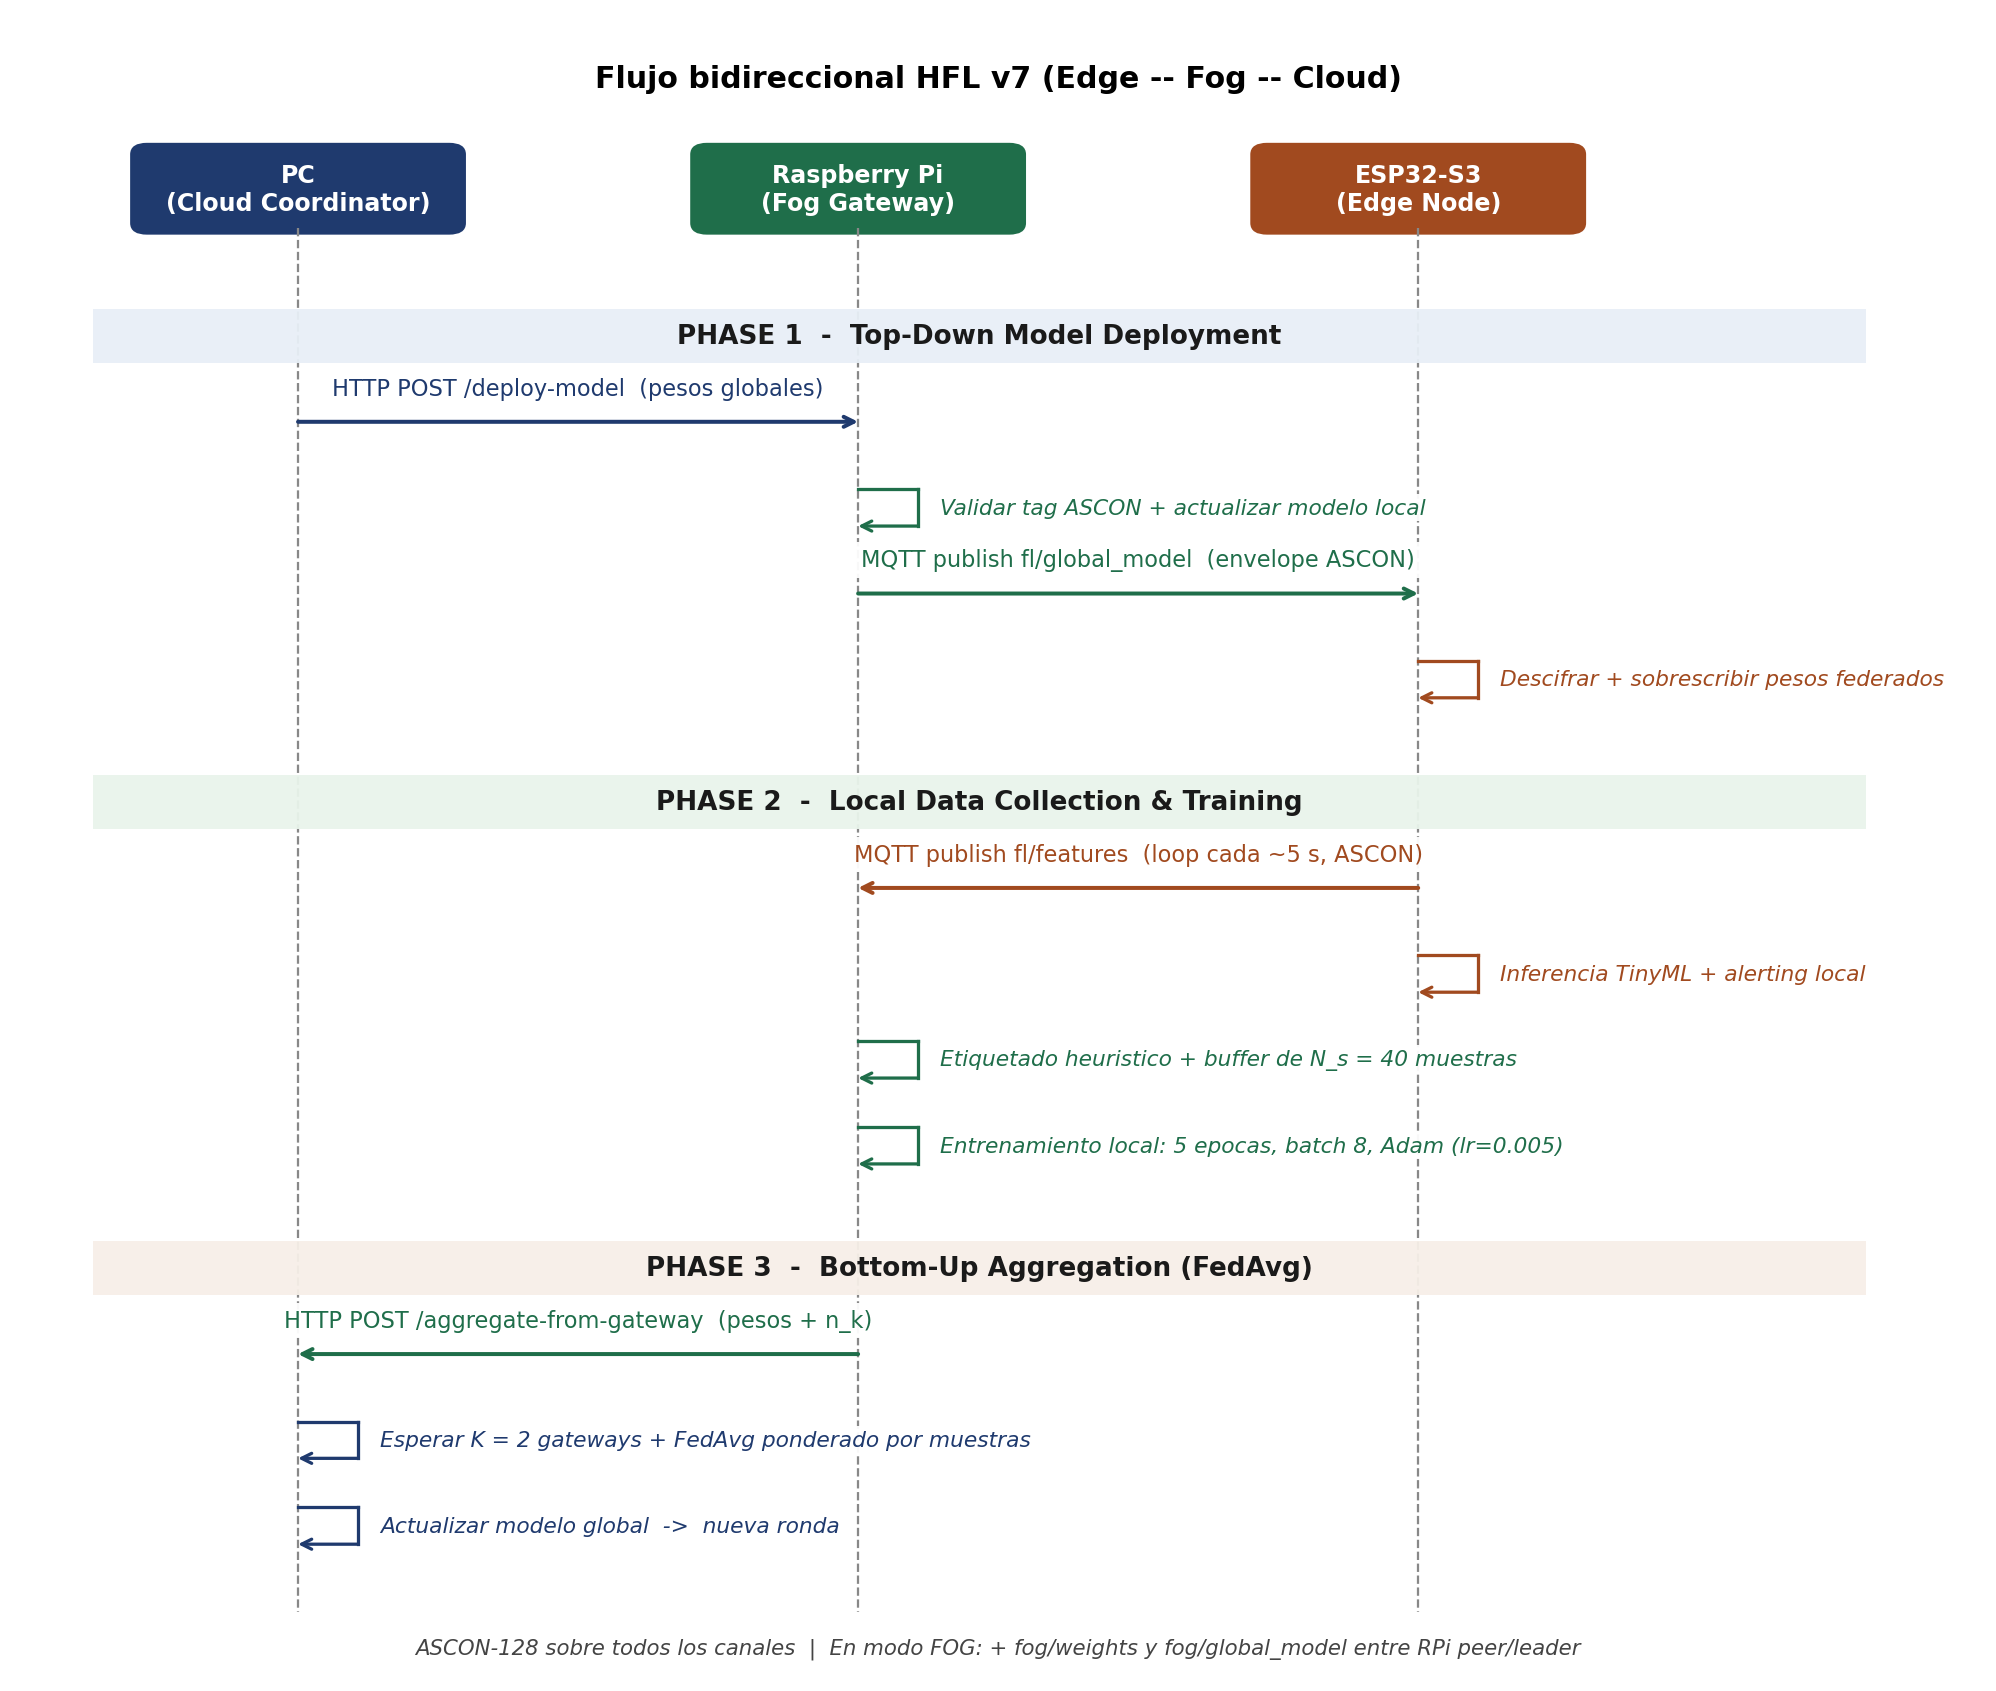
\includegraphics[width=0.92\textwidth]{images/Metodologia/hfl_v7_bidirectional_flow.png}
    \caption{Diagrama de secuencia del protocolo HFL v7 bidireccional. Los actores PC (Cloud), Raspberry Pi (Fog) y ESP32-S3 (Edge) intercambian mensajes en tres fases: despliegue del modelo global, recolección de features con entrenamiento local y agregación FedAvg. Todos los canales MQTT/HTTP se protegen con ASCON-128 cuando la variante está habilitada; en modo FOG se añaden los topics \texttt{fog/weights} y \texttt{fog/global\_model} entre Raspberry Pi peer y leader.}
    \label{fig:hfl_v7_bidirectional_flow}
\end{figure}

En modo FOG, el flujo agrega dos canales adicionales: \texttt{fog/weights} para que los peers envíen pesos al líder y \texttt{fog/global\_model} para que el líder redistribuya el modelo global a los peers.

El etiquetado en el gateway se realiza mediante una \textbf{función heurística} calibrada con las distribuciones estadísticas reales de los datasets:

\begin{itemize}
    \item Si $\texttt{num\_pkts} \geq 50$ \textbf{y} $\texttt{num\_psh} \geq 10$: etiqueta $= 1$ (\texttt{bruteforce}).
    \item Si $\texttt{num\_pkts} \leq 5$ \textbf{y} $\texttt{mean\_pkt\_len} \leq 50$ \textbf{y} $\texttt{num\_psh} \leq 1$: etiqueta $= 2$ (\texttt{scan\_A}).
    \item Si $\texttt{num\_pkts} \leq 30$ \textbf{y} $\texttt{mean\_pkt\_len} \geq 50$: etiqueta $= 0$ (\texttt{normal}).
    \item En otro caso, la muestra se descarta ($-1$).
\end{itemize}

% ====================================================================
\section{Integración de Cifrado Ligero ASCON-128}
\label{sec:ascon}

Para proteger los artefactos de aprendizaje federado en tránsito, se integra \textbf{ASCON-128} \cite{NISTSP8002322025}, el estándar de criptografía ligera seleccionado por NIST para dispositivos restringidos. ASCON provee cifrado autenticado con datos asociados (AEAD), garantizando simultáneamente \emph{confidencialidad} e \emph{integridad} de los mensajes.

\subsection{Parámetros Criptográficos}

\begin{itemize}
    \item \textbf{Clave simétrica:} 128 bits (16 bytes), pre-compartida entre todos los dispositivos.
    \item \textbf{Nonce:} 128 bits, generado a partir de timestamp truncado a 32 bits y un contador monotónico.
    \item \textbf{Tag de autenticación:} 128 bits (16 bytes).
    \item \textbf{Tasa (rate):} 64 bits (8 bytes por bloque).
    \item \textbf{Permutación:} $p^{12}$ para inicialización/finalización, $p^6$ para procesamiento de bloques.
\end{itemize}

Se elige ASCON-128 (rate de 64 bits) sobre la variante ASCON-128a (rate de 128 bits) por dos razones: (i) su mayor número de rondas en la fase de procesamiento del cuerpo proporciona un margen de seguridad superior frente a ataques diferenciales y de cubo recientemente revisados \cite{Kaur2025_ASCON_Survey}; y (ii) los payloads del sistema (features de 13 floats, vectores de pesos de $\sim$3.6\,KB) son lo suficientemente pequeños para que la diferencia de \emph{throughput} entre ASCON-128 y ASCON-128a no sea determinante. Esta decisión es alineada con la recomendación de NIST SP 800-232 para canales con paquetes pequeños \cite{NISTSP8002322025}.

\subsection{Canales Cifrados}

Se cifran los \textbf{cuatro canales de comunicación} del sistema:

\begin{table}[H]
\centering
\caption{Canales de comunicación protegidos con ASCON-128.}
\label{tab:canales_ascon}
\begin{tabular}{l l l l}
\toprule
\textbf{Canal} & \textbf{Protocolo} & \textbf{Contenido} & \textbf{Implementación} \\
\midrule
ESP32 $\to$ RPi & MQTT & Features (13 floats)    & C++ (\texttt{ascon128.h}) \\
RPi $\to$ PC    & HTTP & Pesos locales + métricas & Python (\texttt{ascon128.py}) \\
PC $\to$ RPi    & HTTP & Modelo global            & Python (\texttt{ascon128.py}) \\
RPi $\to$ ESP32 & MQTT & Modelo global            & Python $\to$ C++ \\
\bottomrule
\end{tabular}
\end{table}

El payload cifrado se encapsula en un \emph{envelope} JSON con tres campos codificados en Base64:
\begin{verbatim}
{"ct": "<ciphertext_b64>", "tag": "<tag_b64>", "nonce": "<nonce_b64>"}
\end{verbatim}

\subsection{Métricas de Overhead}

Para cuantificar el overhead de ASCON, se instrumentan todas las operaciones de cifrado y descifrado con temporizadores de alta resolución (\texttt{micros()} en ESP32, \texttt{time.perf\_counter()} en Python) y se registran automáticamente en archivos CSV mediante el módulo \texttt{ascon\_metrics.py}, capturando:

\begin{itemize}
    \item Tiempo de cifrado/descifrado (ms).
    \item Tamaño del plaintext y del envelope cifrado (bytes).
    \item Overhead de comunicación (bytes adicionales y porcentaje).
    \item Ronda de FL asociada.
\end{itemize}

Adicionalmente, se mantiene una \textbf{rama sin cifrado} (\texttt{hfl\_v7-no-ascon}) del repositorio con idéntica funcionalidad pero sin ASCON, permitiendo la comparación directa de tiempos de comunicación como línea base. En esta rama los mensajes se serializan como JSON plano y se registran mediante \texttt{plain\_metrics.py}.

\section{Variantes implementadas en \texttt{hfl\_v7}}
\label{sec:variantes}

\begin{table}[H]
\centering
\caption{Variantes de arquitectura evaluadas.}
\label{tab:variantes_hfl}
\small
\begin{tabular}{l l l l}
\toprule
\textbf{Carpeta} & \textbf{Modelo} & \textbf{Seguridad} & \textbf{Topología} \\
\midrule
\texttt{hfl\_v7-RN} & MLP/RN & ASCON-128 & Estándar y FOG \\
\texttt{hfl\_v7-no-ascon} & MLP/RN & JSON plano & Estándar y FOG \\
\texttt{hfl\_v7-CNN} & CNN-1D & ASCON-128 & Estándar y FOG \\
\bottomrule
\end{tabular}
\end{table}

Estas variantes permiten aislar tres efectos: el impacto del cifrado, el impacto de cambiar el modelo y el impacto de introducir una agregación fog intermedia.

% ====================================================================
\section{Modelos Clásicos de ML como Línea Base}
\label{sec:ml_classic}

Para responder a la pregunta de si TinyML puede alcanzar precisión comparable a modelos tradicionales, se entrenan y optimizan cuatro algoritmos de ML supervisado sobre los mismos datasets:

\begin{enumerate}
    \item \textbf{Decision Tree:} Optimizado con \texttt{GridSearchCV} sobre \texttt{max\_depth}, \texttt{min\_samples\_split}, \texttt{min\_samples\_leaf} y \texttt{criterion}. Incluye \texttt{class\_weight='balanced'} para manejar el desbalance de clases.

    \item \textbf{Random Forest:} Optimizado con \texttt{RandomizedSearchCV} ($n=80$ iteraciones) sobre \texttt{n\_estimators}, \texttt{max\_depth}, \texttt{max\_features} y variantes de \texttt{class\_weight}.

    \item \textbf{Logistic Regression:} Evaluada con penalizaciones L1, L2 y ElasticNet, variando el parámetro de regularización $C$.

    \item \textbf{Support Vector Machine (SVM):} Se comparan kernel lineal y RBF. Para el kernel RBF, se aplica submuestreo estratificado (máximo 25\,000 muestras por clase) para evitar tiempos de entrenamiento prohibitivos.
\end{enumerate}

Todos los modelos se evalúan con validación cruzada estratificada ($k=5$) usando F1-Score macro como métrica de selección. Para estimar la viabilidad de despliegue en ESP32, se utiliza la biblioteca \texttt{m2cgen} para exportar los modelos entrenados a código C puro, y se mide:
\begin{itemize}
    \item Tamaño estimado en memoria del modelo exportado.
    \item Tiempo de inferencia promedio (100 iteraciones con warmup).
    \item Métricas: Accuracy, F1 macro, F1 weighted, Precision, Recall y MCC (Matthews Correlation Coefficient).
\end{itemize}

% ====================================================================
\section{Protocolo Experimental}
\label{sec:protocolo}

La evaluación se organiza en cinco escenarios experimentales:

\subsection{Escenario 1: Sistema HFL Completo con ASCON}

Se despliega el sistema completo en hardware real:
\begin{itemize}
    \item 2 × ESP32-S3 (nodo normal + nodo simulado).
    \item 1 × Raspberry Pi 4 (gateway, broker MQTT, entrenamiento local).
    \item 1 × PC (servidor federado, dashboard).
    \item Red Wi-Fi local compartida.
    \item ASCON-128 habilitado en todos los canales.
\end{itemize}

Se ejecutan $\geq 50$ rondas de aprendizaje federado, registrando accuracy global, loss, tiempos de cifrado/descifrado y tamaños de mensajes.

\subsection{Escenario 2: Sistema HFL sin ASCON (Baseline)}

Idéntico al Escenario 1 pero con ASCON deshabilitado, utilizando la rama \texttt{hfl\_v7-no-ascon}. La comunicación se realiza en JSON plano. Se miden los mismos indicadores para calcular el overhead atribuible exclusivamente al cifrado.

\subsection{Escenario 3: Sistema HFL con CNN-1D}

Se ejecuta la misma arquitectura HFL, pero sustituyendo el MLP por una CNN-1D. En este caso, las capas Conv1D y BatchNorm fusionadas permanecen fijas en el ESP32, mientras que las capas densas finales se actualizan mediante FL.

\subsection{Escenario 4: Estrategia FOG}

Se despliega \texttt{gateway\_hfl\_fog.py} con roles \texttt{leader} y \texttt{peer}. El líder agrega pesos locales y pesos de peers mediante FedAvg fog, envía una actualización preagregada al PC y redistribuye el modelo global hacia peers y ESP32.

\subsection{Escenario 5: Modelos Clásicos Centralizados}

Los modelos clásicos (Sección~\ref{sec:ml_classic}) se entrenan de forma centralizada en el PC usando la totalidad del dataset, con partición 80/20 estratificada. Esto establece un techo de rendimiento (\emph{upper bound}) contra el cual comparar la precisión del sistema federado.

\subsection{Métricas de Evaluación}

\begin{itemize}
    \item \textbf{Precisión de detección:} Accuracy, F1-Score (macro y weighted), Precision, Recall, MCC.
    \item \textbf{Overhead criptográfico:} Tiempo de cifrado/descifrado (ms), incremento de tamaño (bytes, \%), overhead como porcentaje del ciclo total de FL.
    \item \textbf{Eficiencia federada:} Número de rondas hasta convergencia, accuracy por ronda, costo de comunicación por ronda.
    \item \textbf{Viabilidad edge:} Huella de memoria del modelo (KB), tiempo de inferencia en ESP32 ($\mu$s), consumo de SRAM.
    \item \textbf{Efecto de variantes:} comparación entre MLP/RN, CNN-1D, baseline sin ASCON y topología FOG.
\end{itemize}
